\documentclass{article}

\renewcommand{\familydefault}{\sfdefault}

\usepackage{epcc}
\usepackage{graphics}
\usepackage{todonotes}
\usepackage{amsmath}

\usepackage{xcolor}
\usepackage{float} 
\usepackage{pgfgantt}
\usepackage[backend=biber]{biblatex}
\addbibresource{references.bib}
%\usepackage{booktabs}


\renewcommand{\labelenumii}{\theenumii}
\renewcommand{\theenumii}{\theenumi.\arabic{enumii}.}
% this will make nested numbering all arabic numbers

% This example file shows how a report can be laid out using Latex. It
% does not use any special local features so should be portable to other
% places.
% 
% When producing draft copies of a thesis you may want to print only
% selected pages of the thesis. To do this use the command
% 
% dvips -f -p 4 -n 3 myfile.dvi | lpr
% 
% where -p 4 means start printing at page 4 (ie the page that will be
% numbered 4, not necessarily the 4th page) and -n 3 means print 3 pages.
% This example will print pages 4, 5 and 6.
% 
% If you want to print the report and also save paper you can print more
% than one page on each sheet of paper. Use the command
% 
% dvips -f myfile.dvi | psnup -2 | lpr
% 
% to print 2 pages per sheet. psnup can take values 2, 4, 8, or 9.
%
% To produce a PDF version you can create a PostScript copy first
%
% dvips -f myfile.dvi > myfile.pdf
%
% and then convert it
%
% distill myfile.ps
%
% or you can go straight to PDF
%
% pdflatex myfile
%
% Note that pdflatex expects all included figures to be in PDF too. See
% the includegraphics command below.


% This document contains many cross-references and forward references,
% eg in constructing a table of contents, so Latex may need to be run
% twice to get all the references correct. If you need to run Latex twice
% you may get the warning:
% 
% LaTeX Warning: Label(s) may have changed. Rerun to get cross-references right.


\begin{document}

\indentedparagraphing
% remove this ^ line for a "modern" look of paragraphs, where the paragraphs are always separated byt about half-line width and are not indented

\title{\rmfamily Benchmarking the PETSc OpenMP Backend
 \\%
	\vspace{1em} \large{\sffamily Feasibility Study}
}

\author{Leyan Li B293319} % Change to your name here
\date{}


\makeEPCCtitle
\thispagestyle{empty}

\newpage
\pagenumbering{arabic}


%%%%%%%% Preliminaries %%%%%%%%



%%%%%%%% Technical part %%%%%%%%
\section{Introduction}\label{s:intro}


The Portable, Extensible Toolkit for Scientific Computation (PETSc) is a widely used library for large-scale scientific computing, particularly for solving sparse linear systems arising from the discretisation of partial differential equations \cite{petsc_balay2019}. 
It provides scalable data structures and solvers and is widely applied in simulation-based workloads such as fluid dynamics and structural mechanics.

Traditionally, PETSc has relied on MPI for parallel execution. 
While highly effective on distributed-memory systems, this approach can become less efficient on modern many-core architectures with complex NUMA and cache hierarchies. 
On systems such as ARCHER2, using one MPI process per core may increase communication overhead and exacerbate memory contention \cite{archer2_hardware}.
Hybrid MPI+OpenMP execution offers an alternative by combining distributed-memory parallelism across nodes with shared-memory parallelism within a node. 
In principle, this can reduce communication overhead and improve memory utilisation, but performance depends strongly on how rank--thread configurations align with hardware topology, including NUMA locality and cache sharing \cite{judge2022mpiopenmp}.

PETSc has recently introduced an OpenMP backend, making it important to evaluate whether hybrid execution provides consistent and practical performance benefits. 
This project benchmarks the PETSc OpenMP backend on ARCHER2 and compares it with MPI-only execution, aiming to identify when hybrid parallelism is beneficial and which architectural factors determine performance.

The remainder of this report is organised as follows. 
Section~2 reviews the relevant background on parallel programming models and architecture-aware performance. 
Section~3 presents preliminary experiments and initial findings. 
Section~4 defines the project proposal and research questions, followed by the workplan, resource estimation, risk analysis, and a provisional outline of the dissertation.

\section{Background and Literature Review}

\subsection{Parallel Programming Models in HPC}

Parallel applications on modern high-performance computing (HPC) systems are typically implemented using either distributed-memory or shared-memory models. 
MPI is the dominant model for distributed-memory parallelism, while OpenMP is commonly used for shared-memory parallelism within a node. 
Hybrid programming, which combines MPI and OpenMP, has become increasingly important as HPC systems evolve towards many-core architectures.

Beyond these widely adopted models, alternative programming paradigms such as Partitioned Global Address Space (PGAS) have also been developed. 
PGAS approaches, including languages and libraries such as Chapel and OpenSHMEM, provide a global memory abstraction while retaining awareness of data locality, offering a different trade-off between programmability and performance \cite{chapel,openshmem}. 
However, these models are not the focus of this work. 
This project instead concentrates on MPI, OpenMP, and their hybrid use, as PETSc is fundamentally based on MPI and the central objective is to evaluate the effectiveness of its OpenMP backend on ARCHER2.
\subsection{Limitations of Flat MPI}

MPI enables scalable parallel applications, but the traditional ``flat MPI'' approach (one process per core) can become inefficient on modern systems. 
As the number of MPI processes increases, communication overhead grows and contention for shared resources, such as memory bandwidth, becomes more significant \cite{judge2022mpiopenmp}. 
Memory available per process is also reduced, which can further limit performance.

These limitations are particularly evident on systems such as ARCHER2, where each node contains 128 cores and a complex NUMA memory hierarchy \cite{archer2_hardware}  as shown in Figure~\ref{fig:archer2_architecture}. 
In such environments, increasing the number of MPI processes does not necessarily improve performance.

\subsection{Hybrid MPI+OpenMP Programming}

Hybrid MPI+OpenMP programming addresses the limitations of flat MPI discussed in the previous section, 
in particular the increasing communication overhead and resource contention as the number of MPI processes grows.
By using fewer MPI processes and exploiting intra-node parallelism through OpenMP threads, 
hybrid approaches can reduce communication volume, improve memory utilisation, and better match the hierarchical structure of modern HPC systems \cite{judge2022mpiopenmp}.

Previous studies show that hybrid approaches can improve strong scaling for certain applications, including PETSc-based solvers \cite{lange_petsc_hybrid}. 
More recently, PETSc has introduced support for OpenMP-based kernels within its main development branch, 
providing a configurable OpenMP backend (e.g. via the \texttt{--with-openmp-kernels} option), 
which enables explicit investigation of thread-level parallelism within PETSc itself \cite{petsc_openmp_backend}. 
This development makes it particularly important to evaluate whether hybrid execution provides practical performance benefits in real applications.

However, performance is highly application-dependent and requires careful tuning of rank--thread configurations. 
Excessive threading can degrade performance due to increased synchronisation overhead, reduced cache locality, and contention for shared resources such as memory bandwidth. 
In particular, multiple threads within a process may compete for the same memory subsystem, which can limit scalability in bandwidth-bound workloads \cite{numa_tuning,topology_placement}.

\subsection{Node-Level Architecture and NUMA Effects}

Modern HPC nodes are typically based on Non-Uniform Memory Access (NUMA) architectures, where memory access latency depends on the location of data relative to the executing core. 
On ARCHER2, each node consists of two AMD EPYC 7742 processors, providing 128 cores organised into multiple NUMA regions, with cores sharing different levels of cache.

\begin{figure}[h]
    \centering
    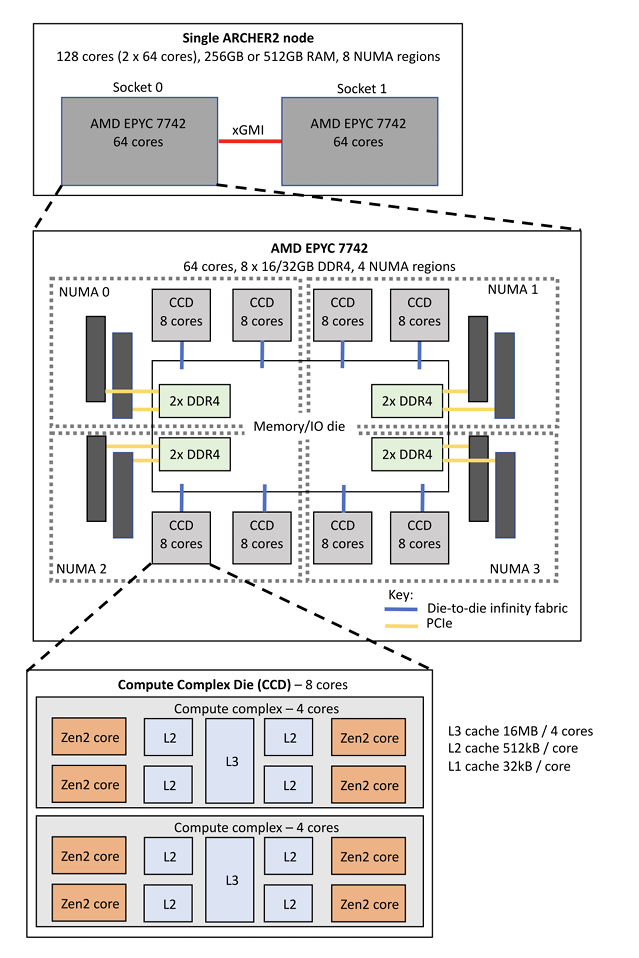
\includegraphics[width=0.5\textwidth]{archer2.png}
    \caption{Architecture of an ARCHER2 node, consisting of two 64-core AMD EPYC 7742 processors.}
    \label{fig:archer2_architecture}
\end{figure}

Figure~\ref{fig:archer2_architecture} illustrates the node-level architecture of ARCHER2, including the organisation of cores, NUMA domains, and cache hierarchy. 
This hierarchical structure has important implications for parallel performance, as memory access costs and cache sharing behaviour vary across different regions of the node.

These architectural features strongly influence application performance. 
In particular, process and thread placement, as well as alignment with hardware topology, are critical factors \cite{numa_tuning,topology_placement}. 
Confining threads within a NUMA region and preserving cache locality are commonly recommended strategies for reducing remote memory access and improving efficiency.

These considerations will be used later to interpret the performance behaviour observed in the experimental results.

\subsection{PETSc and Parallel Linear Solvers}

PETSc is a widely used framework for large-scale scientific computing, particularly for solving sparse linear systems arising from the discretisation of partial differential equations \cite{petsc_balay2019,petsc1997}. 
It provides scalable data structures and a comprehensive range of solvers and preconditioners, enabling efficient solution of large-scale problems on parallel architectures.

Historically, PETSc has been designed around MPI-based distributed-memory parallelism, using domain decomposition and communication patterns that scale to large numbers of processes. 
This makes it well suited to traditional HPC systems, but also means that its performance characteristics are closely tied to the behaviour of MPI, including the limitations of flat MPI discussed in Section~2.2.

More recently, PETSc has introduced support for OpenMP-based kernels within its main development branch, enabling hybrid MPI+OpenMP execution through a configurable OpenMP backend \cite{petsc_openmp_backend}. 
However, this support is currently limited to selected computational kernels rather than the entire codebase. 
As a result, the extent to which PETSc can effectively exploit thread-level parallelism depends not only on the chosen configuration, but also on how extensively OpenMP is utilised within the underlying implementation.

This partial adoption of OpenMP introduces additional complexity in understanding performance behaviour, as improvements from hybrid execution may be constrained by non-parallelised regions or imbalanced workload distribution across threads.

\subsection{Summary and Research Gap}

Existing work suggests that hybrid MPI+OpenMP execution can improve performance by reducing communication overhead and better exploiting node-level parallelism. 
However, these benefits are not universal and are known to depend strongly on application characteristics, problem size, and hardware architecture.

In the case of PETSc, the introduction of an OpenMP backend provides new opportunities for hybrid execution, but also raises additional questions. 
Since OpenMP support is currently limited to selected computational kernels, it remains unclear to what extent PETSc can effectively exploit thread-level parallelism in practice, and to what degree observed performance reflects actual OpenMP utilisation rather than theoretical potential.

Furthermore, there is limited understanding of how the PETSc OpenMP backend performs on modern many-core systems such as ARCHER2, and under which rank--thread configurations it delivers consistent and reproducible performance improvements. 
Prior studies highlight the importance of topology-aware configuration, but do not fully address how these factors interact with partial thread-level parallelism within PETSc.

This project addresses these gaps by systematically benchmarking MPI-only and hybrid configurations on ARCHER2, analysing performance in relation to hardware topology, configuration choices, and the effective utilisation of OpenMP parallelism. 
In addition, it will explore opportunities to further exploit or extend threading within PETSc, particularly in dominant computational kernels.
\section{Preliminary Investigations and Findings}

To evaluate the parallel performance of PETSc in a high-performance computing environment, a set of preliminary experiments was conducted. 
These experiments focused on comparing MPI-only and hybrid MPI+OpenMP execution modes, 
with the aim of observing scalability characteristics under different parallel configurations, identifying potential performance bottlenecks, and assessing whether the PETSc OpenMP backend effectively utilises thread-level parallelism in practice.


\subsection{Experimental Environment and Configuration}

All experiments were carried out on the UK national supercomputing platform ARCHER2, which consists of 5,860 nodes with a total of 750,080 cores. 
Each node contains two AMD EPYC 7742 processors (64 cores at 2.25\,GHz per processor) \cite{archer2_hardware}.

The Cray Programming Environment with the GNU toolchain (\texttt{PrgEnv-gnu/8.4.0}) was used, with \texttt{gcc/11.2.0} as the compiler and \texttt{cray-mpich/8.1.27} as the MPI implementation. 
The system modules also include architecture-specific optimisations (e.g. \texttt{craype-x86-rome}) and performance libraries such as \texttt{cray-libsci}.

The application is based on the PETSc \texttt{ex2} benchmark (located in \texttt{src/ksp/ksp/tutorials/ex2.c}), which constructs a sparse linear system arising from a 2D five-point finite difference discretisation and solves it using a Krylov subspace (KSP) solver with PETSc's parallel matrix and vector interfaces. 
A problem size of $800 \times 800$ was used, corresponding to $640{,}000$ unknowns in total. 
This relatively small problem size was chosen for initial validation of parallel behaviour; larger problem sizes will be considered in later stages to obtain more stable scaling characteristics.

PETSc was configured with OpenMP support enabled using the following key options:

\begin{itemize}
    \item \texttt{--with-openmp=1}
    \item \texttt{--with-openmp-kernels=1}
\end{itemize}
PETSc version 3.24.4 was used.
Compilation was performed using the Cray compiler wrappers (\texttt{cc}, \texttt{CC}, \texttt{ftn}) with optimisation flags (\texttt{-O3}) and debugging disabled. 
This configuration enables OpenMP parallelism in supported computational kernels, while maintaining compatibility with MPI-based distributed-memory execution.

Two execution modes were considered:

\begin{itemize}
    \item \textbf{MPI-only mode}: scalability is evaluated by increasing the number of MPI processes (ranks);
    
    \item \textbf{Hybrid mode (MPI+OpenMP)}: combinations of MPI ranks and OpenMP threads (rank--thread configurations) are evaluated under fixed or varying total core counts.
\end{itemize}

All experiments were submitted using Slurm job scripts to control resource allocation and runtime parameters. 
An example of job scripts is available in \cite{petsc_scripts_repo}. 
Initial tests were restricted to a single node in order to minimise the impact of inter-node communication and focus on intra-node behaviour.


\subsection{Experimental Design}

The experimental study consists of two main components:

\paragraph{MPI-only strong scaling}

In MPI-only mode, the number of MPI processes is increased (e.g., 1, 2, 4, 8, 16, 32, 64, 128), 
and execution time is measured. 
Speedup and parallel efficiency are defined as:

\begin{equation}
S(p) = \frac{T(1)}{T(p)}
\end{equation}

\begin{equation}
E(p) = \frac{S(p)}{p} = \frac{T(1)}{p \cdot T(p)}
\end{equation}

where $T(1)$ is the execution time on a single core and $T(p)$ is the execution time using $p$ cores.
All speedup values are computed relative to the MPI-only single-core baseline (1 rank, 1 core).

\paragraph{Hybrid configuration testing}

In hybrid mode, experiments are performed under the constraint of a single node (128 cores). Configurations are selected such that:

\[
\text{ranks} \times \text{threads} = \text{total cores}, \quad \text{total cores} \leq 128
\]

This ensures full utilisation of available resources. Example configurations include:

\[
(128 \times 1), (64 \times 2), (32 \times 4), (16 \times 8), (8 \times 16), \dots
\]

Execution times are compared across configurations to analyse the impact of different parallel strategies under identical total core counts, and to observe performance trends introduced by OpenMP.

In addition to the single-node study, a limited multi-node comparison was performed at a fixed total core count of 128. 
This was designed as an initial test of whether the relative behaviour of MPI-only and hybrid configurations changes once inter-node communication is introduced. 
Representative thread counts of 1, 2, 4, and 8 were evaluated on 1, 2, and 4 nodes. 
Because the total core count is held constant, this comparison isolates the effect of node distribution rather than overall parallel scaling. 
To better quantify this effect, an additional normalised runtime metric was used:

\begin{equation}
R_{\mathrm{norm}}(n) = \frac{T(n)}{T(1)}
\label{eq:rnorm}
\end{equation}

where \(T(n)\) is the mean runtime on \(n\) nodes for a given thread count, and \(T(1)\) is the corresponding mean runtime on 1 node for the same thread count. 
This metric isolates the effect of node distribution at fixed total core count: values below 1 indicate an improvement relative to the corresponding 1-node case, while values above 1 indicate degradation.

\subsection{Results and Initial Observations}

\begin{figure}[H]
    \centering
    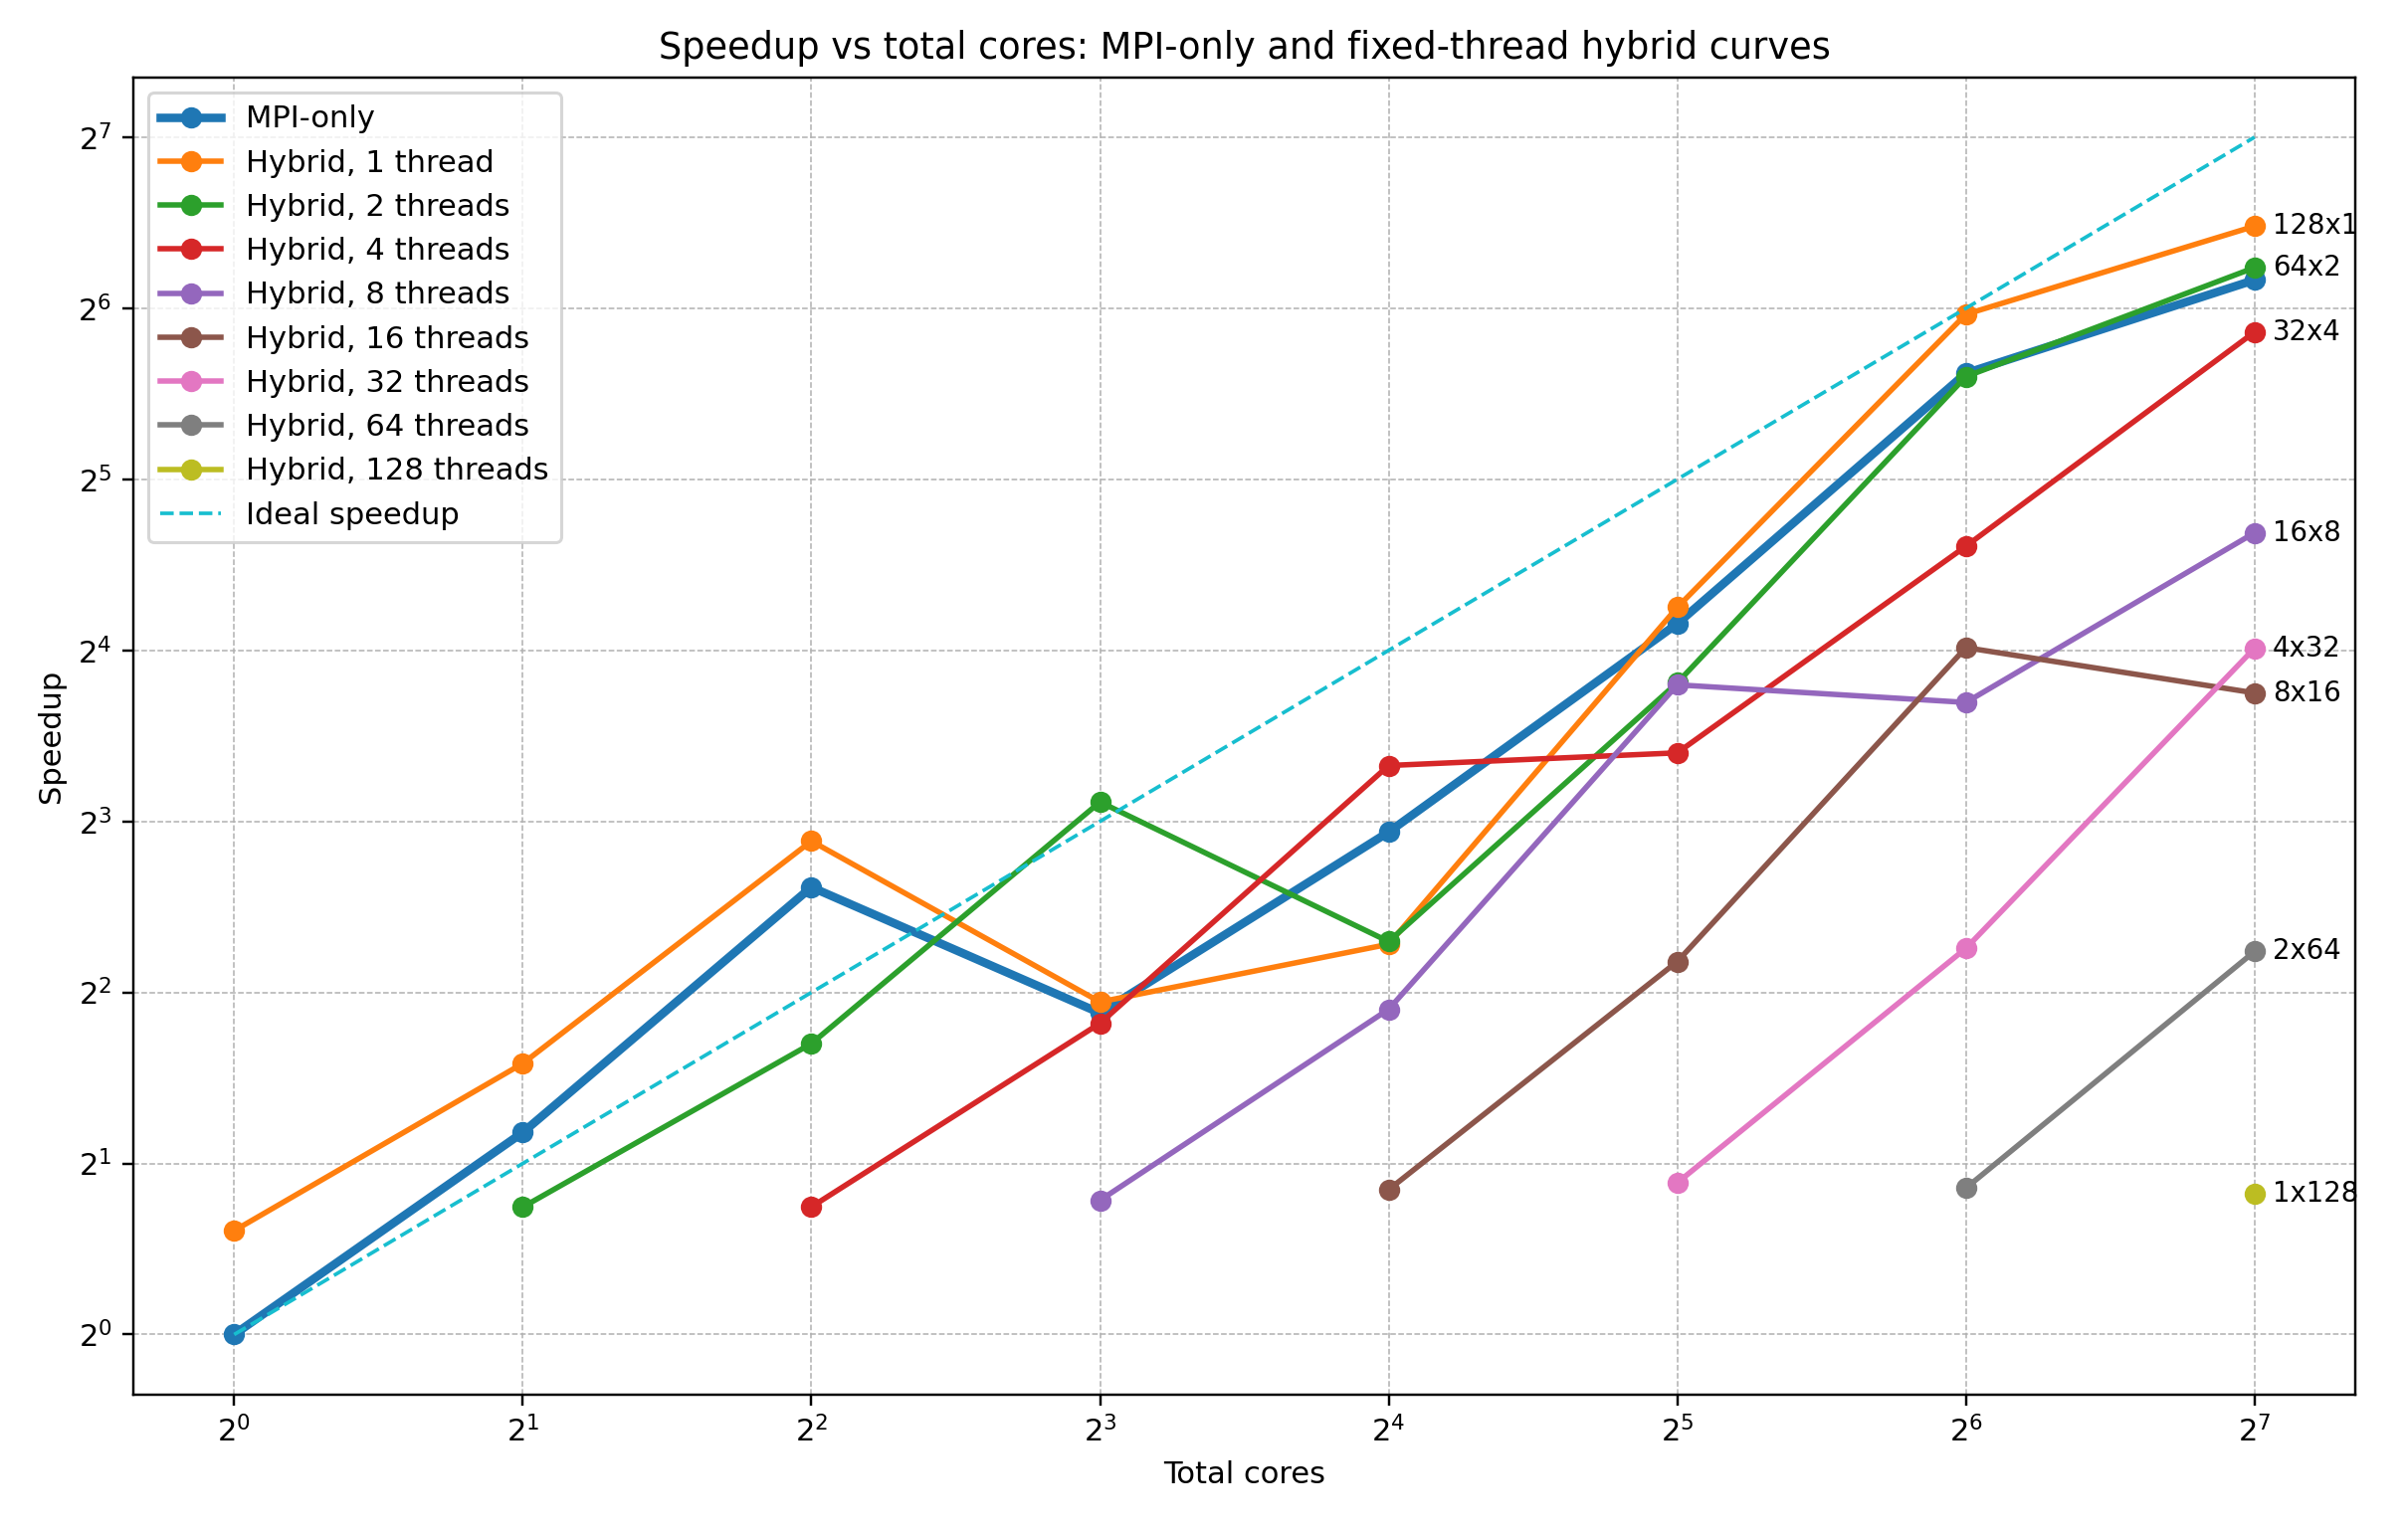
\includegraphics[width=0.75\linewidth]{speedup.png}
    \caption{Speedup of PETSc ex2 benchmark on a single ARCHER2 node under different MPI and hybrid configurations.}
    \label{fig:speedup}
\end{figure}

Figure~\ref{fig:speedup} shows that the speedup behaviour varies substantially across different MPI-only and hybrid configurations. 
This indicates that the performance of the PETSc \texttt{ex2} benchmark on a single ARCHER2 node is highly sensitive to the chosen rank--thread configuration, rather than being determined by core count alone.

All speedup values are computed relative to a common baseline, namely MPI-only execution on a single core (1 rank, 1 thread). 
This definition is important when interpreting the hybrid curves. 
In particular, the first point on a threaded configuration already uses multiple cores, so its initial speedup is expected to be close to the corresponding core count. 
Therefore, the fact that some threaded curves appear to begin near a speedup of 2 does not by itself imply that hybrid execution is inherently more efficient than MPI-only execution; rather, it primarily reflects the use of more than one core relative to the single-core baseline.

Among the hybrid configurations, moderate thread counts show the most promising behaviour. 
The 2-thread configuration performs well across much of the tested range and exceeds MPI-only performance at several points, including 8 and 128 total cores. 
The 4-thread configuration is also competitive at some core counts, although its advantage is less consistent. 
By contrast, configurations with larger thread counts, particularly 8 threads and above, show weaker scalability and lower speedup. 
At very high thread counts such as 32, 64, or 128 threads per rank, performance degrades substantially.

Another notable feature is that the scaling behaviour is not strictly monotonic. 
In several cases, speedup decreases at particular core counts before increasing again. 
This suggests that performance is influenced not only by the total number of cores, but also by how a given rank--thread configuration maps onto the underlying hardware topology. 
In other words, different configurations with the same total core count can still produce substantially different performance. 
Taken together, the single-node results suggest that moderate levels of threading can be beneficial, likely because they reduce MPI overhead without introducing excessive intra-process contention, whereas aggressive threading introduces additional costs that degrade performance.

\paragraph{Initial multi-node comparison.}

To provide a first indication of multi-node behaviour, additional experiments were performed on 2 and 4 nodes while keeping the total core count fixed at 128. 
Representative thread counts of 1, 2, 4, and 8 were selected. 
Rather than constituting a full scaling study, this comparison was intended to examine whether the relative behaviour of MPI-only and hybrid configurations changes once inter-node communication is introduced.

\begin{figure}[H]
    \centering
    \begin{minipage}[t]{0.49\linewidth}
        \centering
        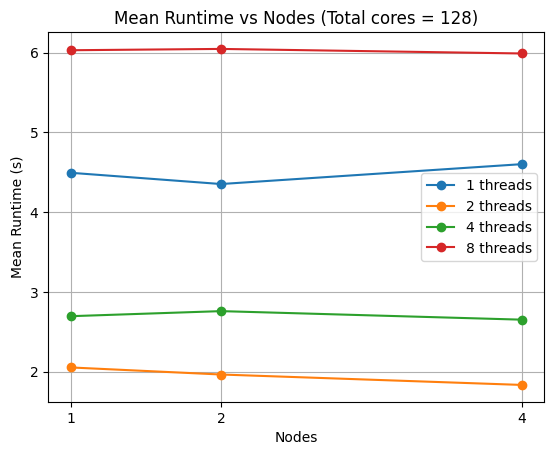
\includegraphics[width=\linewidth]{meanRuntimeNodes.png}
    \end{minipage}\hfill
    \begin{minipage}[t]{0.49\linewidth}
        \centering
        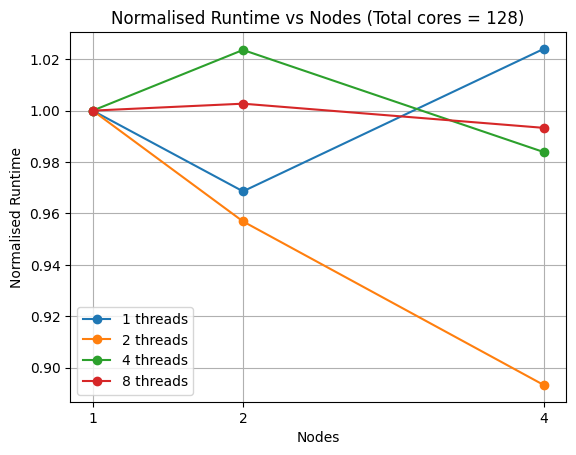
\includegraphics[width=\linewidth]{NorMeanNodes.png}
    \end{minipage}
    \caption{Initial multi-node comparison at fixed total core count of 128. Left: mean runtime versus number of nodes for selected thread counts. Right: normalised runtime relative to the corresponding 1-node case for each thread count.}
    \label{fig:multinode_comparison}
\end{figure}

Figure~\ref{fig:multinode_comparison} complements the single-node observations by showing how selected configurations behave once the same total number of cores is distributed across multiple nodes. 
The left-hand plot shows absolute runtime, while the right-hand plot shows normalised runtime, defined as in Equation~\ref{eq:rnorm} relative to the corresponding 1-node result for each thread count.

In absolute runtime terms, the 2-thread configuration performs best across 1, 2, and 4 nodes, and its runtime decreases further as the computation is distributed across more nodes. 
The 4-thread configuration remains competitive but is less stable, while the 8-thread configuration remains substantially slower and shows no clear advantage. 
MPI-only execution (1 thread per rank) remains relatively stable on 1 and 2 nodes, but becomes slightly slower on 4 nodes.

The normalised runtime results make the cross-node behaviour more explicit. 
The 2-thread configuration shows the clearest improvement, decreasing to approximately 0.89 on 4 nodes, which suggests that reducing the number of MPI ranks may be beneficial once inter-node communication is introduced. 
By contrast, the MPI-only configuration increases slightly above 1 on 4 nodes, indicating mild degradation relative to its own 1-node baseline. 
The 4-thread and 8-thread configurations remain closer to 1, suggesting that they gain comparatively little from distributing the computation across additional nodes under this fixed-core setup.

Taken together, these results suggest that moderate hybrid configurations remain effective beyond the single-node case and may become more favourable than MPI-only execution when communication extends across nodes. 
Although this is only a limited fixed-core comparison, it provides preliminary support for the hypothesis that reducing the number of MPI ranks can help mitigate communication overhead in multi-node environments.

\subsection{Preliminary Analysis and Problem Identification}

To interpret the observed performance differences, profiling analysis was conducted using Linaro MAP (version 25.0.4) to examine runtime behaviour and the utilisation of OpenMP parallelism. 
The profile shown here corresponds to a representative hybrid configuration using 8 MPI processes with 8 OpenMP threads per process (64 cores in total) on a single node. 
This configuration was selected as it lies within the practical range identified in Section~3.3 and provides a useful case for examining thread-level behaviour.

\begin{figure}[H]
    \centering
    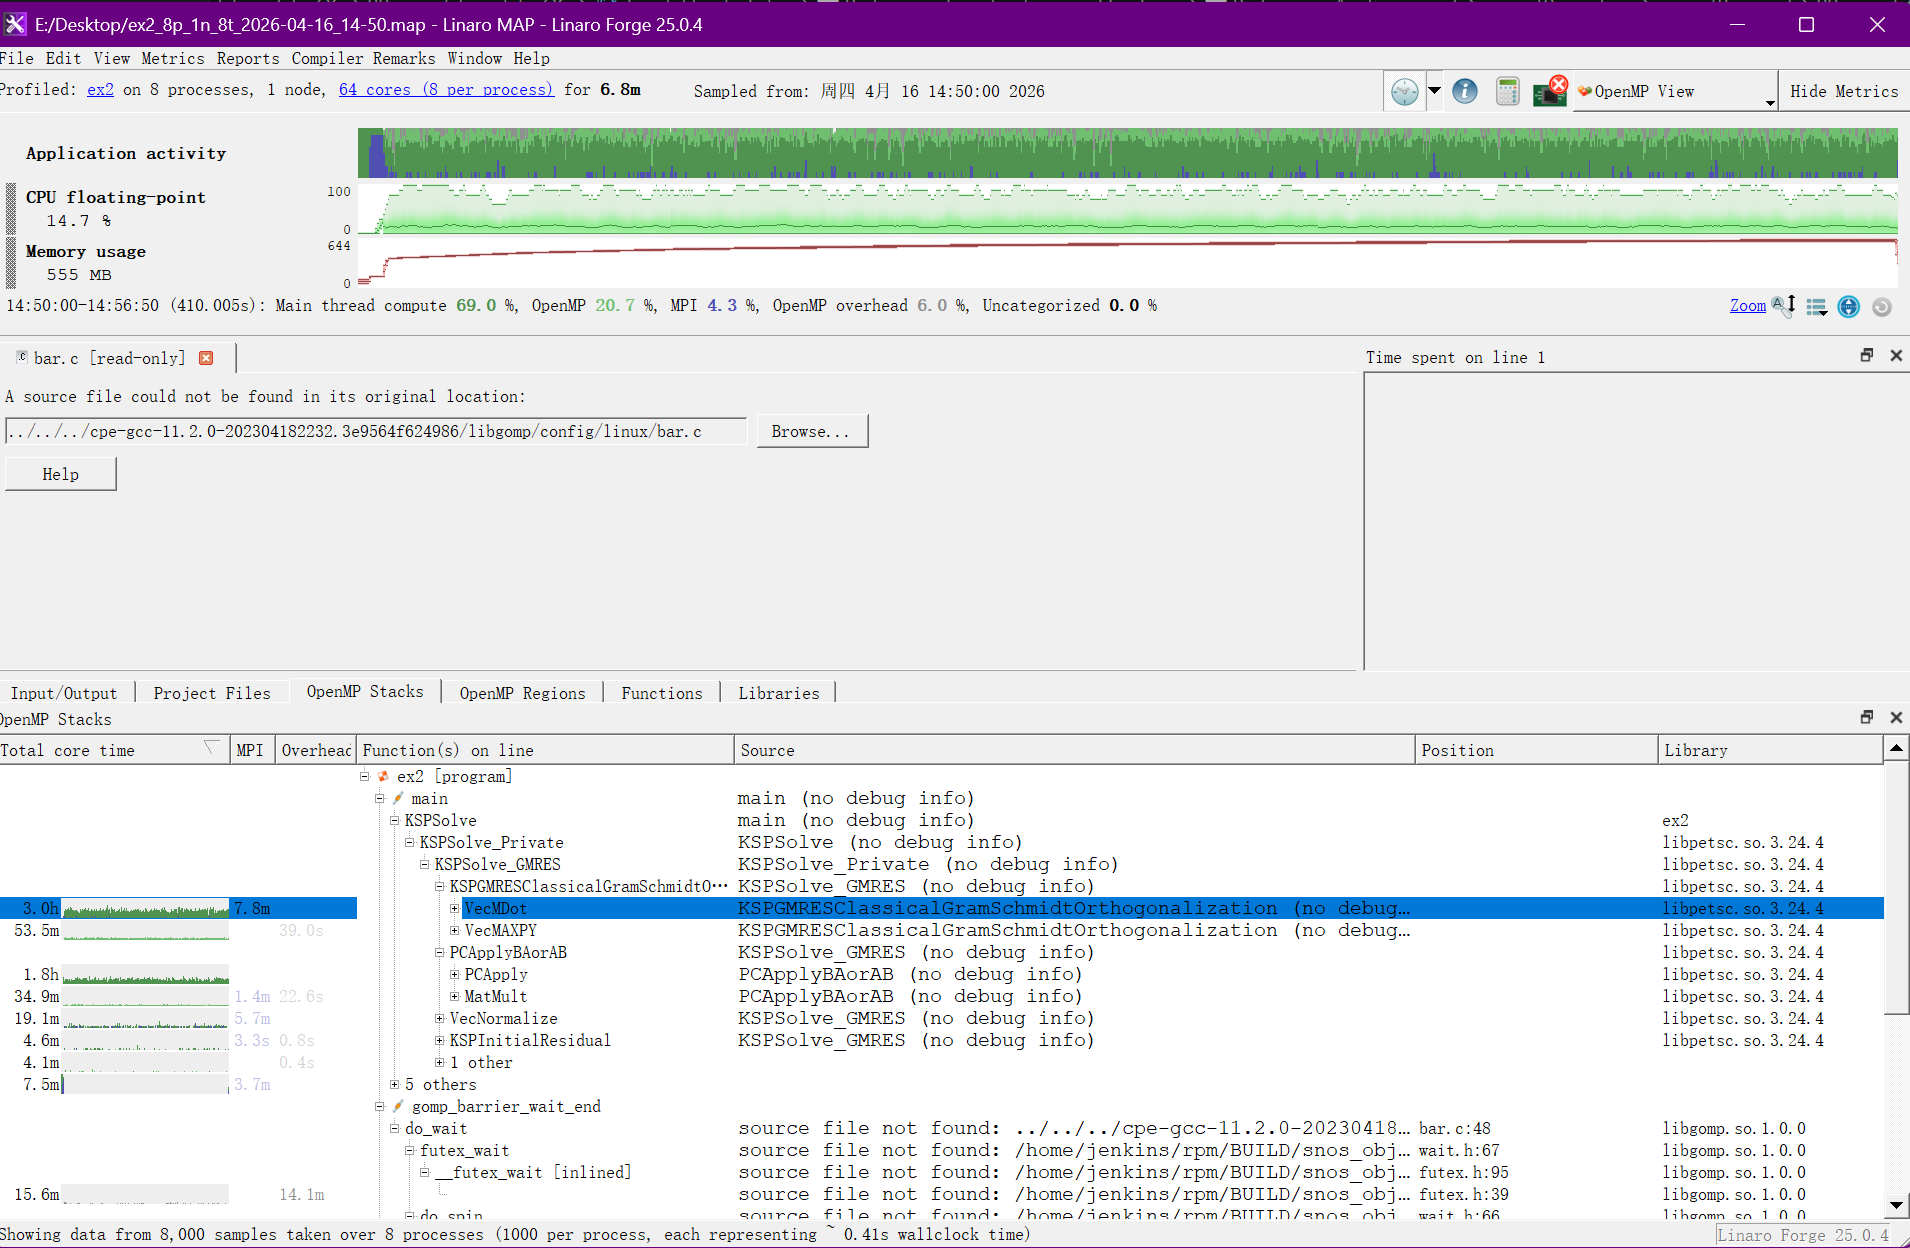
\includegraphics[width=0.9\linewidth]{map_overview.png}
    \caption{Linaro MAP profile showing overall execution breakdown, including MPI, OpenMP, and serial computation.}
    \label{fig:map_overview}
\end{figure}

As shown in Figure~\ref{fig:map_overview}, the PETSc OpenMP backend is active during execution. 
Approximately 20\% of total runtime is spent in OpenMP regions, with an additional overhead of around 6\%. 
However, a substantial proportion of execution, close to 70\%, remains in the main thread. 
This indicates that while thread-level parallelism is present, it is not dominant.

To understand this behaviour in more detail, the distribution of time across computational routines was analysed.

\begin{figure}[H]
    \centering
    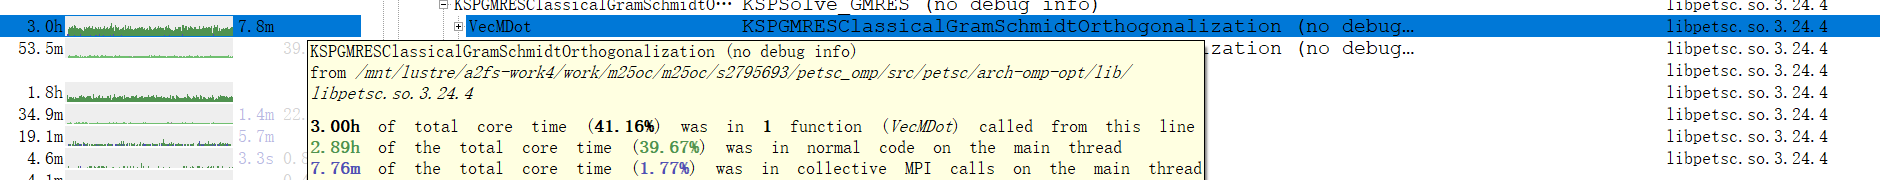
\includegraphics[width=0.9\linewidth]{vecdot.png}
    \caption{Profiling breakdown showing that \texttt{VecMDot} dominates execution time.}
    \label{fig:map_hotspot_vecmdot}
\end{figure}

Figure~\ref{fig:map_hotspot_vecmdot} shows that the function \texttt{VecMDot} accounts for over 40\% of total execution time, making it the dominant computational kernel. 
The majority of this time is spent in normal code on the main thread, with only a negligible proportion attributed to MPI or parallel execution. 
This indicates that \texttt{VecMDot} does not effectively exploit OpenMP parallelism under the current configuration.


\begin{figure}[H]
    \centering
    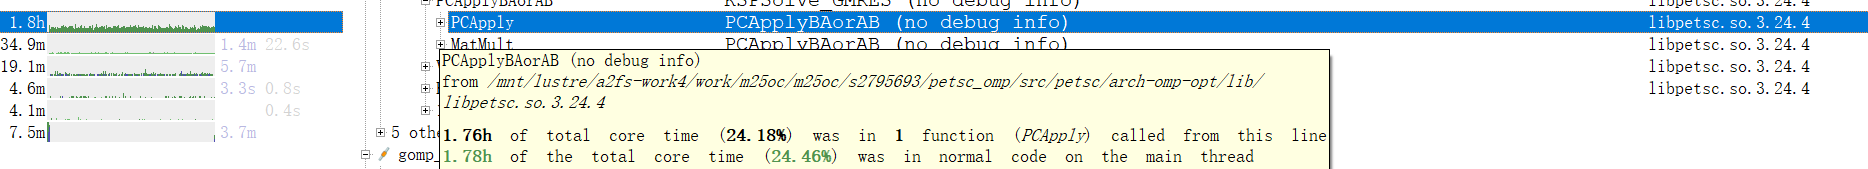
\includegraphics[width=0.9\linewidth]{pcapply.png}
    \caption{Profiling breakdown showing the contribution of \texttt{PCApply} to total execution time.}
    \label{fig:map_hotspot_pcapply}
\end{figure}

In addition to \texttt{VecMDot}, other functions also contribute significantly to total runtime. 
For example, as shown in Figure~\ref{fig:map_hotspot_pcapply}, the function \texttt{PCApply} accounts for approximately 24\% of execution time and similarly executes predominantly on the main thread, with limited evidence of effective OpenMP utilisation.

Taken together, these results indicate that although OpenMP regions are present at the application level, key computational kernels are not consistently parallelised. 
As a result, overall performance is limited by an uneven distribution of work, where a significant fraction of execution remains effectively serial.

These observations help explain the performance trends observed in Section~3.3. 
Moderate thread counts (e.g., 2 or 4 threads per process) can provide performance improvements by reducing MPI communication overhead, while still maintaining reasonable resource utilisation. 
However, increasing the number of threads does not lead to proportional gains, as important computational routines remain serial and threads may compete for shared resources such as memory bandwidth.

Overall, the performance of PETSc \texttt{ex2} on ARCHER2 is influenced not only by parallel configuration, but also by the extent to which OpenMP parallelism is effectively utilised within dominant computational kernels. 
The presence of partially serial regions suggests that further performance improvements would require better parallelisation of key routines such as \texttt{VecMDot} and \texttt{PCApply}.

\subsection{Implications for Further Work}

The preliminary experiments demonstrate that hybrid parallel performance on ARCHER2 is strongly dependent on both hardware architecture and the effective utilisation of OpenMP parallelism. 
Increasing thread count alone does not guarantee performance improvement. 
Instead, moderate thread configurations (particularly 2 or 4 threads per process) provide a better balance between communication overhead, memory locality, and resource utilisation.

The profiling analysis in Section~3.4 further shows that performance is limited not only by architectural factors, but also by incomplete parallelisation within key computational routines. 
In particular, the function \texttt{VecMDot} dominates execution time while not being effectively parallelised, indicating a clear bottleneck in the current implementation.

Based on these findings, subsequent work will focus on a more detailed investigation of representative rank--thread configurations within a practical range. 
The current results already suggest that configurations with 1, 2, 4, and 8 threads per process provide a useful reduced configuration set for both node-level and initial multi-node analysis.

Further work will include:

\begin{itemize}
    \item extending the profiling analysis to quantify the utilisation of OpenMP parallel regions and identify additional bottlenecks;
    
    \item investigating whether key computational kernels (e.g. \texttt{VecMDot}) can be optimised or better parallelised;
    
    \item comparing different compiler environments (e.g. \texttt{PrgEnv-gnu} and \texttt{PrgEnv-cray}) to evaluate their impact on hybrid performance;
    
    \item extending the current limited multi-node comparison into a broader scaling study across additional problem sizes and node counts.
\end{itemize}

\section{Project Proposal}\label{s:proposal}

This project investigates whether the recently introduced OpenMP backend in PETSc 
can provide meaningful and reproducible performance benefits 
over traditional MPI-only execution on modern many-core NUMA architectures such as ARCHER2.
Rather than asking whether hybrid parallelism is universally better, 
the project aims to determine under which conditions the OpenMP backend is effective, 
when it is not, and which architectural factors explain the observed behaviour.

\subsection{Research Questions and Hypotheses}

Building on the preliminary findings in Section~3, 
the dissertation will address the following research questions.

\vspace{0.5em}

\noindent\textbf{RQ1: Can the PETSc OpenMP backend deliver practically useful performance improvements over MPI-only execution on modern CPU nodes?}

This question evaluates not only runtime reduction, but also speedup, parallel efficiency, reproducibility, and overall practical usefulness.

\textbf{H1:} Compared with MPI-only execution, moderately hybrid MPI+OpenMP configurations are expected to achieve better performance by reducing the number of MPI ranks and lowering communication overhead.

This advantage may become more visible in multi-node settings, where inter-node communication becomes more significant.
\vspace{0.8em}

\noindent\textbf{RQ2: If performance benefits exist, under which rank--thread configurations do they occur?}

This question aims to identify stable and repeatable configurations that perform well, and to examine how optimal configurations vary with problem size and node count.

\textbf{H2:} The best performance is expected at moderate thread counts (particularly around 2--4 threads per rank), while higher thread counts may degrade performance due to increased overhead and pressure on shared resources.
\vspace{0.8em}

\noindent\textbf{RQ3: What are the main sources of performance limitation in the PETSc OpenMP backend, and can these limitations be improved?}

This question investigates not only communication and architectural factors, but also whether key computational routines are effectively parallelised in practice. In particular, it examines whether dominant kernels limit overall performance and whether their parallel performance can be improved.

\textbf{H3:} Performance limitations are expected to arise not only from architectural factors and runtime overheads, but also from incomplete and uneven parallelisation within key computational routines. In particular, dominant kernels (e.g. \texttt{VecMDot} and \texttt{PCApply}) are likely to limit the overall benefit of hybrid execution, and improving their parallel performance may lead to better overall scalability.
\vspace{0.8em}

\noindent\textbf{RQ4: How general are the observed performance trends?}

This question examines whether the results remain consistent across different problem sizes, node counts, compiler environments, and solver types.

\textbf{H4:} Performance benefits from the OpenMP backend are expected to be conditional rather than universal, depending on problem size, hardware topology, solver behaviour, and runtime environment.


\subsection{Success Criteria}

The project will be considered successful if it achieves the following objectives:

\begin{enumerate}
    \item it provides a systematic and reproducible evaluation of performance, including clear measurements of runtime, speedup, and parallel efficiency across a representative range of MPI-only and hybrid configurations;

    \item it explains the observed performance trends using profiling-based evidence, with particular attention to communication overhead, threading costs, and key computational bottlenecks that limit the effective utilisation of OpenMP parallelism;

    \item it validates these trends across multiple problem sizes and both node-level and multi-node settings, ensuring that the conclusions are robust and not limited to a specific configuration;

    \item it produces practical and reproducible guidance for configuring PETSc on ARCHER2.
\end{enumerate}

A stronger outcome would additionally include comparison across compiler environments (e.g. \texttt{PrgEnv-gnu} and \texttt{PrgEnv-cray}), as well as deeper profiling-based analysis of performance bottlenecks and runtime behaviour.


\subsection{Minimum Viable Product and Fallbacks}

\subsubsection{Minimum Viable Product}

If time or resources are limited, the minimum viable outcome is a systematic benchmark study on ARCHER2 comparing MPI-only execution with a representative subset of hybrid configurations. 
Where feasible, and as already suggested by the preliminary fixed-core comparison, this will also include a limited multi-node study on a small set of representative configurations, in order to test whether the observed single-node trends remain valid once communication extends across nodes.

At minimum, the study will include configurations with 1, 2, 4, and 8 threads per process, together with stable measurements of runtime, speedup, and efficiency.

In addition, basic profiling analysis will be used to identify major performance bottlenecks (e.g. dominant kernels such as \texttt{VecMDot}), even if detailed optimisation is not fully achieved.

These results should be sufficient to determine whether the OpenMP backend provides measurable performance benefits under practical conditions, and to give a basic architectural interpretation of the observed trends. 
This outcome would still allow the project to address the main research questions, particularly RQ1 and RQ2.

\subsubsection{Fallback Strategies}

To ensure deliverability under practical constraints, 
fallback strategies will be applied by prioritising benchmark-based 
analysis if profiling tools prove difficult to use, 
focusing on detailed single-node experiments if multi-node execution is limited, 
treating instability in certain OpenMP configurations as valid and analysable outcomes, 
emphasising complete and reproducible node-level results if larger problem sizes cannot be fully explored, 
and relying on bottleneck identification rather than full optimisation if performance improvements cannot be reliably achieved.

\subsubsection{Possible Extensions}

If the core objectives are achieved early, the project may be extended in several directions:

\begin{itemize}
    \item comparison of compiler environments and runtime settings, including compiler flags, thread affinity, and process mapping strategies;
    
    \item deeper profiling and architectural analysis, including MPI time, thread synchronisation overhead, memory bandwidth usage, and cache behaviour;

    \item further investigation of kernel-level optimisation opportunities, including improving the parallel performance of dominant routines such as \texttt{VecMDot};

    \item evaluation of additional PETSc solvers or problem types to assess the generality of the observed performance trends.
\end{itemize}
%%%%%%%% Project Management part %%%%%%%%

\section{Workplan}\label{s:plan}

At the time of writing, this project is at the feasibility stage. 
Initial benchmarking and profiling have already been conducted, 
providing early insights into performance behaviour. 
The remaining work focuses on refining these results, extending the experimental study, 
and producing a complete and well-supported analysis.

The workplan is structured as a sequence of interrelated tasks, 
where early results are validated and used to guide subsequent experiments and analysis.

\subsection{Main Tasks}

The remaining work is organised into four main components.

\begin{itemize}

    \item \textbf{Single-Node Validation and Refinement} \\
    Repeat selected single-node experiments under controlled conditions, extend the study to larger problem sizes, and confirm the consistency of the main performance trends. 
    This stage will be used to identify a reduced set of representative rank--thread configurations for the later study. 
    Where useful, it may also include limited exploration of alternative PETSc sparse matrix formats (e.g. \texttt{AIJSELL} or \texttt{SELL}), compiler environments, or related systems such as Cirrus, in order to test whether the observed trends depend strongly on implementation choices or platform.

    \item \textbf{Multi-Node Benchmarking} \\
    Build on the initial fixed-core multi-node comparison by evaluating selected MPI-only and hybrid configurations across multiple nodes (e.g. 2--8 nodes). 
    The aim is to determine whether the advantages of moderate hybrid configurations persist once communication costs increase, and to assess how sensitive the conclusions are to node count and problem size.

    \item \textbf{Profiling, Kernel Analysis, and Limited Optimisation} \\
    Use profiling tools (e.g. Linaro MAP) to quantify MPI, OpenMP, and serial execution time, identify dominant kernels (such as \texttt{VecMDot} and \texttt{PCApply}), and examine the extent to which OpenMP is effectively exploited. 
    Where feasible, this stage will also include limited implementation work aimed at improving the parallel performance of dominant routines or related execution paths, followed by testing and benchmarking of any resulting changes.

    \item \textbf{Synthesis and Dissertation Preparation} \\
    Integrate the benchmarking and profiling results into a coherent analysis, validate the main conclusions across problem sizes and node counts, and produce the final dissertation report, figures, and presentation.
\end{itemize}

\subsection{Timeline Overview}

The overall timeline is illustrated in Figure~\ref{fig:gantt}. 
It reflects the fact that only limited progress is expected between the submission of this feasibility report and the end of the examination period, while the majority of the project work will be carried out afterwards.

\begin{figure}[H]
\centering
\resizebox{\textwidth}{!}{%
\begin{ganttchart}[
    y unit title=0.5cm,
    y unit chart=0.6cm,
    x unit=0.25cm,
    vgrid,
    hgrid,
    time slot format=isodate,
    bar/.append style={fill=blue!50},
    milestone/.append style={fill=red}
]{2026-04-01}{2026-08-20}

\gantttitlecalendar{month=shortname} \\

\ganttbar[bar/.append style={fill=blue!30}]{Feasibility / presentations / exams}{2026-04-18}{2026-05-31} \\
\ganttbar[bar/.append style={fill=blue!60}]{Single-node refinement}{2026-06-01}{2026-06-30} \\
\ganttbar[bar/.append style={fill=blue!60}]{Multi-node benchmarking}{2026-07-01}{2026-07-31} \\
\ganttbar[bar/.append style={fill=orange!70}]{Profiling / kernel analysis / optimisation}{2026-06-15}{2026-07-31} \\
\ganttbar[bar/.append style={fill=green!40}]{Initial write-up and figures}{2026-06-15}{2026-07-31} \\
\ganttbar[bar/.append style={fill=green!60}]{Final synthesis and writing}{2026-08-01}{2026-08-14} \\

\ganttmilestone{Feasibility}{2026-04-17} \\
\ganttmilestone{Submission}{2026-08-14} \\
\ganttmilestone{Talk}{2026-08-17}

\end{ganttchart}%
}
\caption{Project timeline (Gantt chart). 
Light blue: limited work during the feasibility / exam period. 
Blue: benchmarking. Orange: profiling and optimisation. Green: writing and synthesis. Red: milestones.}
\label{fig:gantt}
\end{figure}

The time schedule is therefore expected to be as follows:

Feasibility report submission: 17 April 2026;

Presentations and examinations: mid-April to end of May;

Single-node validation and refinement: June;

Profiling, kernel analysis, limited optimisation, and parallel write-up: late June to July;

Multi-node benchmarking: July;

Final synthesis, report completion, and submission preparation: early August;

Final submission: 14 August 2026;

Final presentation: week beginning 17 August 2026.


\subsection{Work Strategy}

The project follows an iterative and data-driven workflow, but the later stages are also planned to overlap where appropriate.

The first priority after the examination period will be to consolidate the existing single-node results by repeating selected experiments, extending to larger problem sizes, and confirming the most representative configurations. 
These validated results will then guide the multi-node study, so that the broader benchmark campaign remains focused and manageable rather than exhaustively exploring every possible configuration.

Profiling and limited optimisation work will partly overlap with benchmarking. 
For example, while longer benchmark runs are in progress, intermediate results can already be analysed, figures can be prepared, and initial sections of the dissertation can be drafted. 
Similarly, profiling may identify opportunities for kernel-level improvements that can then be implemented, tested, and benchmarked without waiting for all experimental work to finish.

This overlapping strategy reduces the risk of leaving too much writing until the end of the project, while also ensuring that the final dissertation is informed by validated results rather than by purely speculative planning.



\section{Resources Estimation}

This project relies primarily on CPU-based HPC resources on ARCHER2. 
The estimate is based on the planned number of benchmark configurations, repeated runs, and a conservative allowance for additional experiments, profiling overhead, and failed or repeated jobs.
No special data-access, ethical approval, or NDA requirements are expected for this project.

Table~\ref{tab:resources} summarises the main resource requirements.

\begin{table}[H]
\centering
\begin{tabular}{|l|l|}
\hline
\textbf{Resource} & \textbf{Estimated Requirement} \\
\hline
Compute (CPU) & 700--2000 core-hours \\
\hline
Node usage & 1 node (single-node study), 2, 4, and 8 nodes (multi-node study) \\
\hline
Storage & 5--15 GB (logs, CSV files, profiling outputs) \\
\hline
Software & PETSc, MPI, OpenMP, Linaro MAP, Python \\
\hline
Platform & ARCHER2 (Cray EX system) \\
\hline
\end{tabular}
\caption{Estimated project resources}
\label{tab:resources}
\end{table}

The benchmark campaign is divided into a full single-node configuration study and a selected multi-node study.

\paragraph{Single-node configurations.}
For the single-node study, valid rank--thread configurations satisfy:

\[
\text{ranks} \times \text{threads} \le 128
\]

with both ranks and threads selected from \(\{1,2,4,8,16,32,64,128\}\). 
This yields a total of 36 valid configurations.

\paragraph{Multi-node configurations.}
For the multi-node study, node counts of 2, 4, and 8 are considered. 
Thread counts are restricted to \(\{1,2,4,8\}\), reflecting the practical range identified in Section~3.3.

For each node count, configurations are selected such that:

\[
\text{ranks} \times \text{threads} \le 128
\]

and only configurations that utilise all allocated nodes are included (i.e. the number of MPI ranks is sufficient to distribute work across all nodes).

Under these constraints, the number of valid configurations is:

\begin{itemize}
    \item 2 nodes: 22 configurations
    \item 4 nodes: 18 configurations
    \item 8 nodes: 14 configurations
\end{itemize}

giving a total of:

\[
22 + 18 + 14 = 54
\]

multi-node configurations.

\paragraph{Total benchmark configurations.}
Combining both components, the benchmark campaign contains:

\[
36 + 54 = 90
\]

distinct configurations.

To improve robustness, selected configurations may be repeated at larger problem sizes to validate observed trends. 

\paragraph{Runtime estimation.}
To estimate computational cost, a representative runtime per configuration is derived from preliminary measurements. 
Observed runtimes range from approximately 2 seconds at high core counts to over 100 seconds at low core counts, with typical values for most configurations lying between these extremes.

To provide a conservative and realistic estimate, a representative runtime of approximately 10--20 seconds per run is assumed for configurations using up to 128 cores.

Expressed as CPU time, this corresponds approximately to:

\[
128 \times 15 \approx 1920 \text{ core-seconds} \approx 0.5 \text{ core-hours per run}
\]


With 5 repeated runs per configuration and a total of 90 configurations, the baseline benchmark cost is therefore:

\[
90 \times 5 \times 0.5 \approx 225 \text{ core-hours}
\]

\paragraph{Total estimated cost.}
The above estimate accounts only for the planned benchmark runs. 
In practice, additional computational cost will arise from exploratory experiments, profiling runs, repeated or failed jobs, and the implementation and validation of potential optimisations.

Profiling (e.g. using Linaro MAP) introduces non-negligible overhead, while optimisation work typically requires additional benchmarking to assess performance improvements.

To account for these factors, a conservative scaling factor of approximately 3--10 is applied, giving an overall estimate of:

\[
700\text{--}2000 \text{ core-hours}
\]

This estimate reflects a balance between experimental coverage and practical resource constraints, while remaining feasible within the available allocation.

\section{Risk Analysis}

This project depends on HPC resources, experimental results, and analysis tools. 
The main risks are related to resource availability, technical challenges, and time management.

Table~\ref{tab:risks} summarises the key risks, their impact, and mitigation strategies.

\begin{table}[H]
\centering
\begin{tabular}{|p{3.5cm}|p{2cm}|p{2cm}|p{5.5cm}|}
\hline
\textbf{Risk} & \textbf{Probability} & \textbf{Impact} & \textbf{Mitigation} \\
\hline
Limited access to ARCHER2 (queue delays) & Likely & Moderate & Run experiments early; prioritise key configurations; use smaller test cases when needed \\
\hline
System downtime or maintenance on ARCHER2 & Unlikely & Moderate & Use alternative systems (e.g. Cirrus); ensure scripts are portable \\
\hline
Data loss (experimental results or logs) & Possible & Severe & Regularly back up results; store outputs in persistent directories; avoid relying solely on temporary storage \\
\hline
Loss of write-up or report files & Possible & Severe & Use version control (e.g. Git); maintain backups; commit changes regularly \\
\hline
Profiling tools (MAP) difficult to use or unstable & Possible & Moderate & Use simpler timing-based analysis; rely on benchmark trends if profiling fails \\
\hline
Unexpected performance results (no clear improvement) & Likely & Moderate & Treat as valid outcome; focus on analysis and explanation rather than expected improvement \\
\hline
Large problem sizes increase runtime significantly & Likely & Moderate & Select representative sizes; balance accuracy and computational cost \\
\hline
Time constraints before deadlines & Possible & Severe & Begin writing early; overlap benchmarking and analysis; prioritise core results \\
\hline
Errors in scripts or experiment setup & Possible & Moderate & Use incremental testing; validate on small runs before scaling up \\
\hline
\end{tabular}
\caption{Risk assessment and mitigation strategies}
\label{tab:risks}
\end{table}

Most identified risks fall into the medium category, as they are likely to occur but can be mitigated through careful planning. 
The most critical risks relate to time management and potential data or write-up loss, as these can directly affect the ability to complete and submit the project. 
System-level risks related to HPC availability are mitigated through fallback strategies and alternative platforms.

To reduce overall risk, the project follows an incremental and flexible workflow. 
Experiments, analysis, and writing are carried out in parallel, allowing early detection of issues. 
In addition, the minimum viable project (single-node benchmarking with key configurations) ensures that meaningful results can still be delivered even if some risks materialise.


\section{Outline of the Dissertation Report}\label{s:dissertation_outline}

The final dissertation is expected to follow a structure aligned with the research questions and workplan proposed in this report. 
A provisional chapter outline is given below.

\begin{enumerate}

    \item \textbf{Introduction}: 
    Introduces the motivation for studying the PETSc OpenMP backend, defines the project aims, research questions, and scope, and summarises the main contributions.

    \item \textbf{Background and Related Work}: 
    Reviews MPI, OpenMP, and hybrid parallel programming in HPC, discusses NUMA effects, cache hierarchy, and topology-aware performance, and summarises prior work on PETSc and hybrid parallel solvers.

    \item \textbf{Experimental Platform and Methodology}: 
    Describes the ARCHER2 and Cirrus hardware and software environments, the PETSc benchmark and problem setup, and the experimental design, performance metrics, and reproducibility strategy.

    \item \textbf{Single-Node Performance Evaluation}: 
    Presents MPI-only and hybrid benchmark results on a single node, compares rank--thread configurations, and analyses performance trends and configuration sensitivity. 
    This chapter also incorporates profiling-based analysis (e.g. using Linaro MAP) to examine runtime behaviour, identify dominant computational kernels, and assess the effectiveness of OpenMP parallelism. 
    Where applicable, it will additionally explore potential improvements through modifications or optimisation of key kernels and evaluate their impact on performance.

    \item \textbf{Multi-Node Scaling and Analysis}: 
    Extends the single-node study to a multi-node setting, evaluating selected configurations across multiple nodes. 
    The same analytical framework is applied to examine how communication overhead, process placement, and reduced MPI concurrency affect performance. 
    Profiling results are used where appropriate to identify changes in runtime behaviour and emerging bottlenecks in the presence of inter-node communication.

    \item \textbf{Discussion}: 
    Interprets the results in relation to hardware topology and OpenMP utilisation, evaluates how far the research questions and hypotheses are supported, and discusses limitations and possible future work.

    \item \textbf{Conclusion}: 
    Summarises the main findings, provides practical recommendations for configuring PETSc on ARCHER2, and reflects on the effectiveness and limitations of the PETSc OpenMP backend.

\end{enumerate}

\pagebreak
\printbibliography



\end{document}

